\documentclass[a4paper,12pt]{article}
\usepackage[cp1250]{inputenc}
\usepackage[english]{babel}



\usepackage[pdftex]{graphicx}
\usepackage{amsmath}
\usepackage{listings}
\usepackage{xcolor}
\usepackage{color}


\setlength{\textwidth}{6.5in}
\setlength{\oddsidemargin}{0 cm}
\setlength{\evensidemargin}{0 cm}

\begin{document}

\begin{titlepage}
\begin{center}
\large Statistical Inference final assignment\\[1cm]
\LARGE Central limit theorem and  A/B testing\\[1cm]
\large Author: Rok Bohinc \\
\large Basel, June 2019 \\[1 cm]
\end{center}

\begin{abstract}
This work I investigate the distribution of averages of 40 samples from the exponential distribution and show how it compares to the Central Limit Theorem. I show that the mean and variance of the simulated distribution are well approximated with the corresponding theoretical vales. I also show that the simulated distribution is approximately normal.

\end{abstract}
\end{titlepage}


\section{Averages from exponential distribution}

In this project I have investigated the averages of 40 samples from the exponential distribution and compared it with the Central Limit Theorem, i.e. a Gaussian distribution with the appropriate mean and standard deviation. I have performed a thousand simulations of the exponential distribution with the characteristic parameter equal to 0.2. Below is the R code for performing the according simulations.

\footnotesize
\begin{lstlisting}[backgroundcolor = \color{lightgray}, language=R]
n <- 40 # number of samples
l <- 0.2 # characteristic parameter
nsim <- 1000 # number of simulations

data <- matrix(rexp(n*nsim,l), nsim) # sample n*nsim exponentials
means <- apply(data,1,mean) # calculate the mean of each row

meanth1 <- 1/l # theoretical mean for 1 sample
sigmath1 <- 1/l # theoretical standard deviation for 1 sample
meanexp1 <- mean(data[,1]) # simulated mean for 1 samples
sigmaexp1 <- sd(data[,1]) # simulated standard deviation for 1 samples

sigmath40 <- sigmath1/sqrt(n) # theoretical standard deviation for n samples
meanth40 <- meanth1 # theoretical mean for n samples
meanexp40 <- mean(means) # simulated mean for n samples
sigmaexp40 <- sd(means) # simulated standard deviation for n samples

# Show values
round(c(meanth1,sigmath1,meanexp1,sigmaexp1),2)
round(c(meanth40,sigmath40,meanexp40,sigmaexp40),2)

\end{lstlisting}
\normalsize

The code essentially sets the correct values of the parameters, generates random variables from the exponential distribution, calculates the means for a sample size of 40, and evaluates the means and standard deviations for a distribution with a sample size of 1 and 40.

The comparison between the theoretical values of the mean and standard error and the simulated ones is presented in Table \ref{tab:CLT}. The values obtained from the central limit theorem, i.e. mean of 5 and standard deviation of 0.79, are close to the estimated mean and standard deviation of the simulated distribution, which are 5.03 and 0.78, respectively. This implies that the central limit theorem can be well applied for the given exponential parameter and the the sample size. Furthermore, in Figure \ref{fig:CLT} I compare a histogram of 40 averages from the exponential distribution to the normal distribution with according mean and standard deviation. The figure confirms the correctness the application of the central limit theorem.

\newpage
\section{Appendix}

 \begin{table}[!h]
\begin{center}
\caption {\label{tab:CLT} \textbf{Simulated vs. theoretical means and standard error}}
\vspace{0.2 cm}
{\begin{tabular}{|c|c|c|c|c|}
\hline   &  Mean & Standard deviation  \\
\hline           
 Simulated values (1 sample) & 4.88 &  5.19    \\
 Theoretical values (1 sample)    & 5 & 5   \\ 
 \hline     
 Simulated values (40 sample) & 5.05 &  0.81    \\
 Theoretical values (40 sample)    & 5 & 0.79   \\ 
\hline 
\end{tabular} }
 \\
 \vspace{0. cm}
\end{center}
 A comparison between the theoretical means and standard errors and the corresponding simulated values from the exponential distribution for 1000 simulation and for sample sizes 1 and 40. The parameter in the exponential distribution was set to 0.2
\end{table} 

\begin{figure}[!h]
\centering
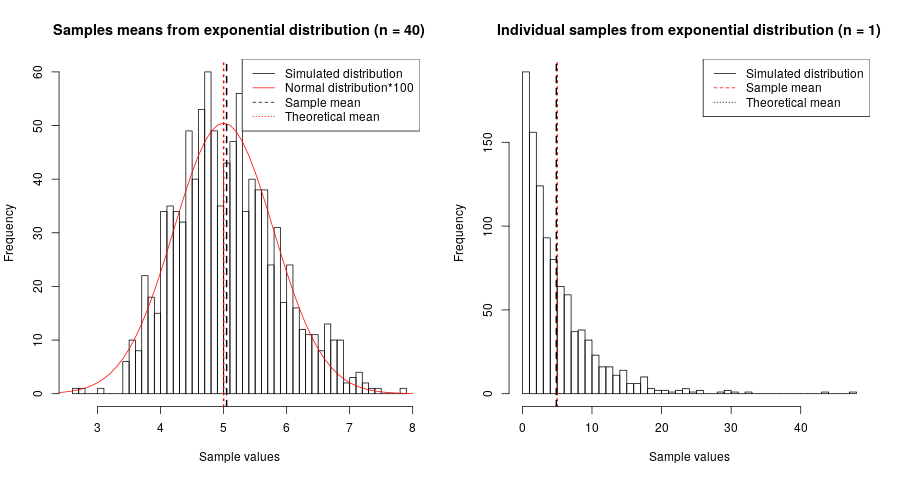
\includegraphics[width=\textwidth]{Means.png}
\caption{ \label{fig:CLT}
Left plot depicts  a comparison between the histogram of simulated means of 40 samples form the exponential distribution (black solid line) and a Gaussian distribution (red solid line). The vertical lines represent the means of the simulated distribution (black dashed line) and the normal distribution (red dotted line). The normal distribution was scaled by 100 to approximately match the counts in the histogram. Right plot depicts a histogram of 1000 simulations from the exponential distribution.}
\end{figure}

\end{document}


